\documentclass[a4paper]{article}

\usepackage{fullpage} % Package to use full page
\usepackage{parskip} % Package to tweak paragraph skipping
\usepackage{tikz} % Package for drawing
\usepackage{amsmath}
\usepackage{hyperref}

\title{SAP Challenge}
\author{Kou Wen}

\begin{document}

\maketitle

\section{Introduction}

The fancy title of SAP Challenge is \emph{Which Novel Do I Belong To?}. Translating the title into machine learning language is classifying the documents into correct categories (text classification). There are quite a mount of classification algorithms which can be applied to solve this issue, e.g. KNN, Logistic regression (For multiple classes, it is preferred as SoftMax), decision tree, linear discriminant analysis, SVM, etc. Those approaches can be regarded as linear approach which assumes the data is linear separable. But if kernel trick is preferred, that is another kind of story. The assumption is that those data is not linear separable that no appropriate hyperplane can be learnt using the above approaches, so kernel trick would seek for another feature space which can linearize the feature from the original feature space to make the problem linear separable again. But in this task, I would like to adopt nowadays fashion approach Convolutional Neural Network aka.\emph{CNN}, since Neural Network will directly solve non linear separable problems; a lot of works have demonstrated \textbf{CNN} will achieve really surprising accuracy and it has been widely applied in industry. In this task, I would like to tackle the different layers: convolutional layers, pooling layers, fully connected layers, etc and manipulate the learnable parameters for example to try how many filters is suitable for each convolutional layers to seek a good CNN structure which can well solve classification problem.

In the \emph{Which Novel Do I Belong To?}, there is another critical issue in feature extraction. The representation of each text is not in natural English word since they have been encrypted so it is not possible to apply any pretrained word embedding as feature directly as other typical text classification problem. But it is said "each character has a deterministic mapping" which means each word e.g. "boy" could always be mapped as "sua", so character level feature extraction can be suitable for this task. X. Zhang \cite{ZhangZL15} demonstrated char level CNN for text classification would achieve similar accuracy compared with word level using word embedding feature.

In section\ref{algoDetail}, the detail of the algorithms is described. In section\ref{exp}, experiments and analysis are explained. In section\ref{conclusion}, conclusion is summarized.

\section{Algorithm Detail}\label{algoDetail}

\subsection{Feature Extraction}
In this task, one-hot feature extraction is applied to encode char in char dictionary:
\begin{equation}
D = \{'a': \mathbf{a},'b': \mathbf{b},'c': \mathbf{c},'d': \mathbf{d}....\}
\end{equation}
For this task, the char dictionary will contain only 26 alphabet characters, so the one-hot feature dimension is $R^{26 \times 1}$.

This one hot representation would make sense since each word including spaces or other will deterministically be mapped to another aphetic space, so the concatenated chars may still contain the semantic meaning though the separation of each independent word can not be really found. In addition, ngram is chosen to represent the article in the raw feature space. To achieve a more robust feature extraction, a few n grams representation of each article will be stacked together.

\subsection{NOVEL CNN}
For novel classification, one uncertain issue to decide the appropriate size of filter in n gram convolutional layer; since the document is encrypted it is difficult to have a proper kernel size. So before the sequential model, a concatenated convolution layers with different kernel size is designed before the sequential model. After the the paralleled concatenated layers, I applied 3 convolutional layers and 2 fully connected layers. The architecture of the \textbf{NOVEL CNN} is shown in Fig.\ref{cnn}.

In addition to control the overfitting issues, a $50$ dropout rate is added after each fully connected layers. The length selection of each text will be mean of the text length in the training corpus. It is believed that the volume of the content in this task will contain enough information for text classification. Gradient descent is applied to perform the optimization.

\begin{figure}
\begin{center}
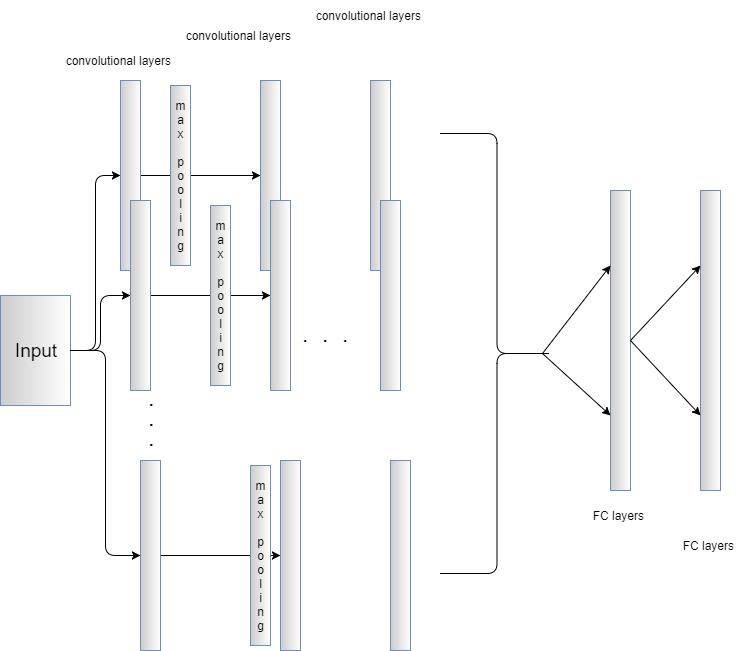
\includegraphics[width=10cm]{CNN_structure.png}
\end{center}
\caption{The structure of CNN for novel classification}\label{cnn}
\end{figure}

\section{Experiment}\label{exp}

The data set contain more 30000 corpus. 80\% will be applied as training set and the rest of the data will be the test. 
\begin{table}
\centering
\begin{tabular}{|c|c|c|}
  \hline
  % after \\: \hline or \cline{col1-col2} \cline{col3-col4} ...
   {} & Training set & Testing set \\
  \hline
  ACC & 90.00 & 74.36 \\
  \hline
\end{tabular}\caption{Experiment result}
\end{table}
\section{Conclusion}\label{conclusion}
The implemented CNN structure would a achieve a enough result. To address the capability of the CNN, comparison with baseline algorithms should be applied e.g. SVM. Beside, another fancy idea may be plausible to solve the encrypted novel is to add one more recurrent layer (LSTM) before CNN layers. The intuition is that the chars have sequential relationship since the content of the novel is from original text with deterministic mapping.

\bibliographystyle{plain}
\bibliography{bibliography.bib}
\end{document}
